Depuis mon intégration du CEA au LC2M en Octobre dans le cadre d'un nouveau postdoc, je m'intéresse à l'influence des défauts nanométriques dans les métaux sur le comportement plastique à l'échelle macroscopique.
Cette étude s'inscrit dans le cadre de la conception des futurs réacteurs à fission et fusion et vise à clarifier les effets de l'irradiation d'aciers sur l'écrouissage, la localisation, la fragilisation, \textit{etc.}
Dans ce contexte, la Dynamique des Dislocations (DD) \cite{Zbib2012_DDD} est un outil numérique qui permet d'étudier l'interaction des dislocations avec les défauts d'irradiation à l'échelle microscopique et de comprendre l'influence sur le comportement à l'échelle du grain.
Néanmoins, la DD requiert, en accord avec la théorie des dislocations, le calcul des actions réciproques entre tous les segments des dislocations discrétisées présentes dans le domaine d'étude.
Il s'en suit que cette méthode est très coûteuse en terme de temps de calcul pour des volumes élémentaires représentatifs contenant un grand nombre de défauts.


\paragraph{Motivations/Objectifs:}
$\newline$
Le Modèle Discret/Continu (DCM) \cite{lemarchand2001_DCM,jamond2016_DCM} permet de contourner les difficutlés liées au coût de calcul caractéristiques des simulations DD.
Dans cette approche, le mouvement des dislocations et les aires que ces dernières balaient sont traduites en terme de déformations plastiques qui sont distribués sur les points de Gauss d'un maillage éléments finis.
Cet étalement de la déformation plastique permet de régulariser la discontinuité du déplacement résultant du mouvement des dislocations.
La résolution éléments finis apparaît alors comme une étape de relaxation visant à équilibrer les déformations plastiques en tenant compte des conditions aux limites.
Toutefois, l'étape de régularisation conduit à une mauvaise estimation du champ de contrainte dans le voisinage des dislocations (pour des distances de l'ordre de la taille du maillage), de sorte qu'une correction provenant de la DD est utilisée localement.
Les contraintes ainsi déterminées donnent accès aux forces de Peach-Köhler dont on déduit l'évolution du réseau de dislocations.

Récemment, une formulation de la DCM dans laquelle une approche de type Transformées de Fourier Rapides (FFT) remplace la méthode des éléments finis a été proposée \cite{bertin2015_fft}.
\begin{figure}[h!]
  \centering
  \subcaptionbox{Configuration initiale \label{subfig:disloc_ini}}{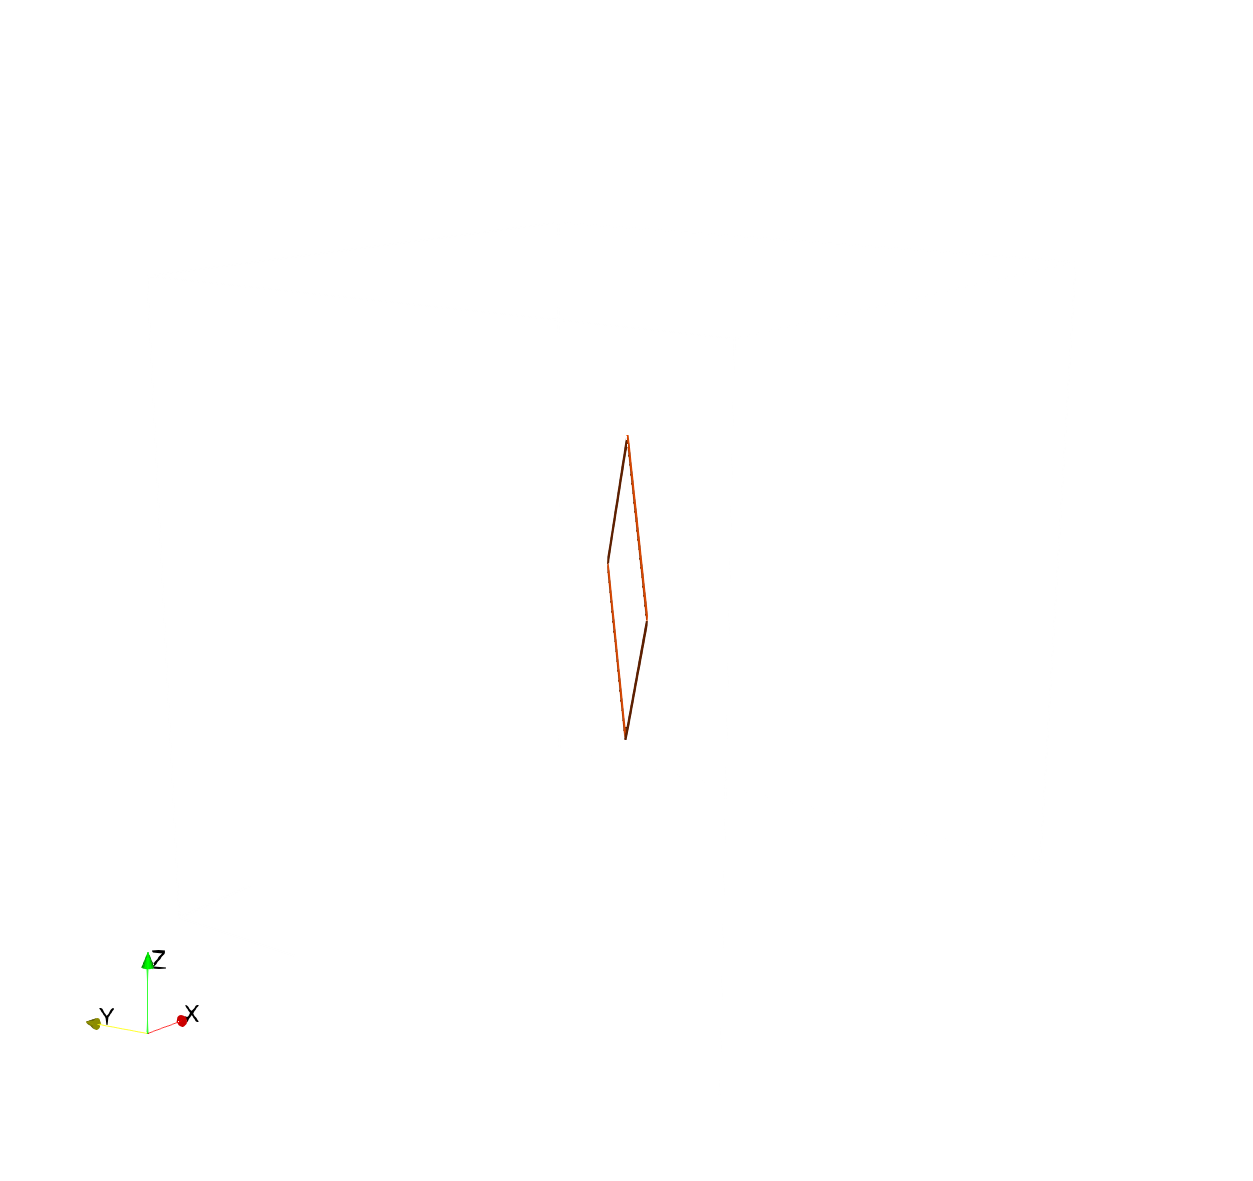
\includegraphics[trim=0 0 0 4cm, clip,height=0.4\textwidth]{pngFigures/initial_disloc.png}}
  \subcaptionbox{Configuration finale \label{subfig:disloc_fini}}{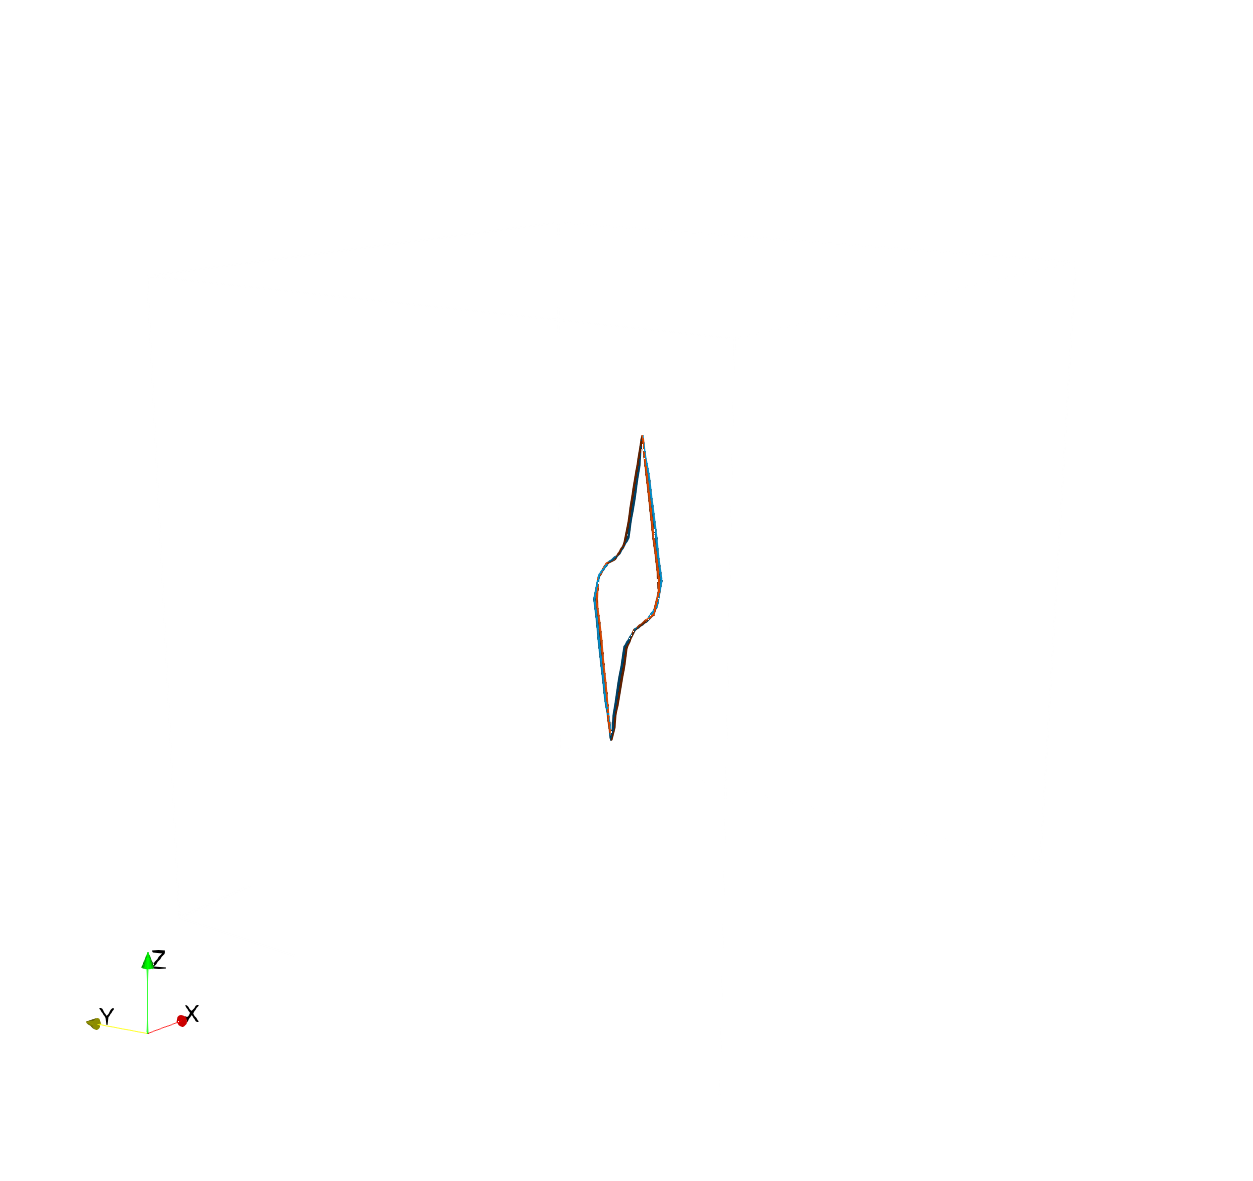
\includegraphics[trim=0 0 0 4cm, clip,height=0.4\textwidth]{pngFigures/final_disloc.png}}
  %\subcaptionbox{Configuration initiale (zoom)\label{subfig:disloc_ini}}{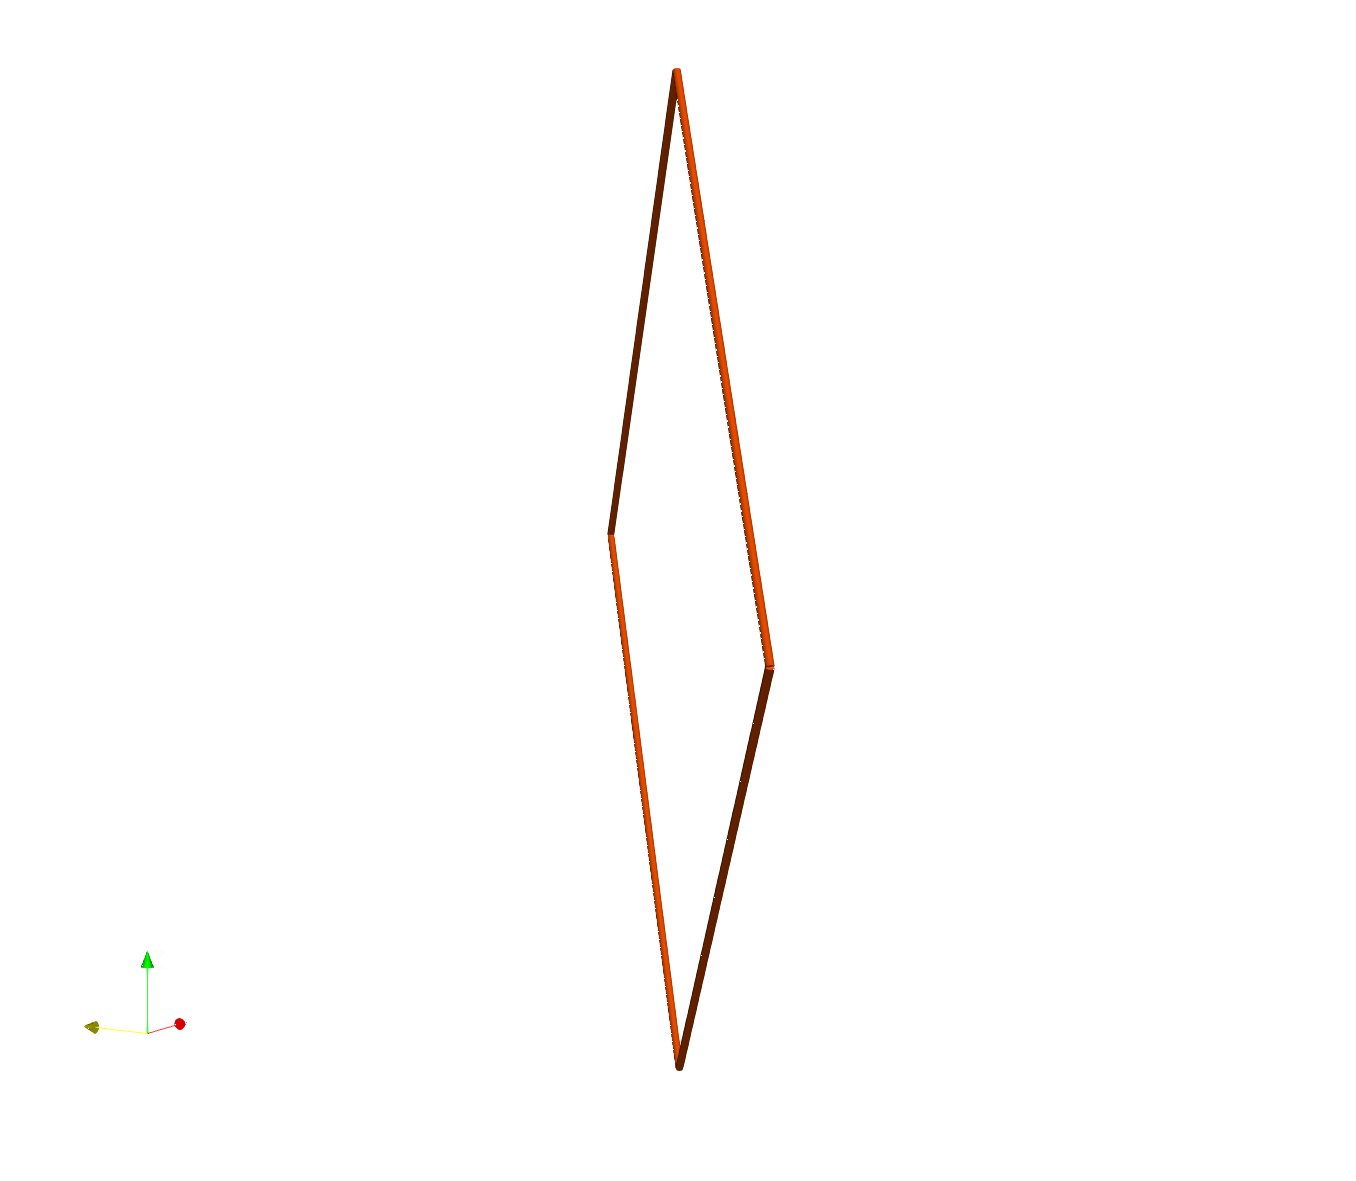
\includegraphics[height=0.4\textwidth]{pngFigures/initial_disloc_zoom.png}}
  %\subcaptionbox{Comparaison des contraintes sur la configuration finale \label{subfig:disloc_fini_stress}}{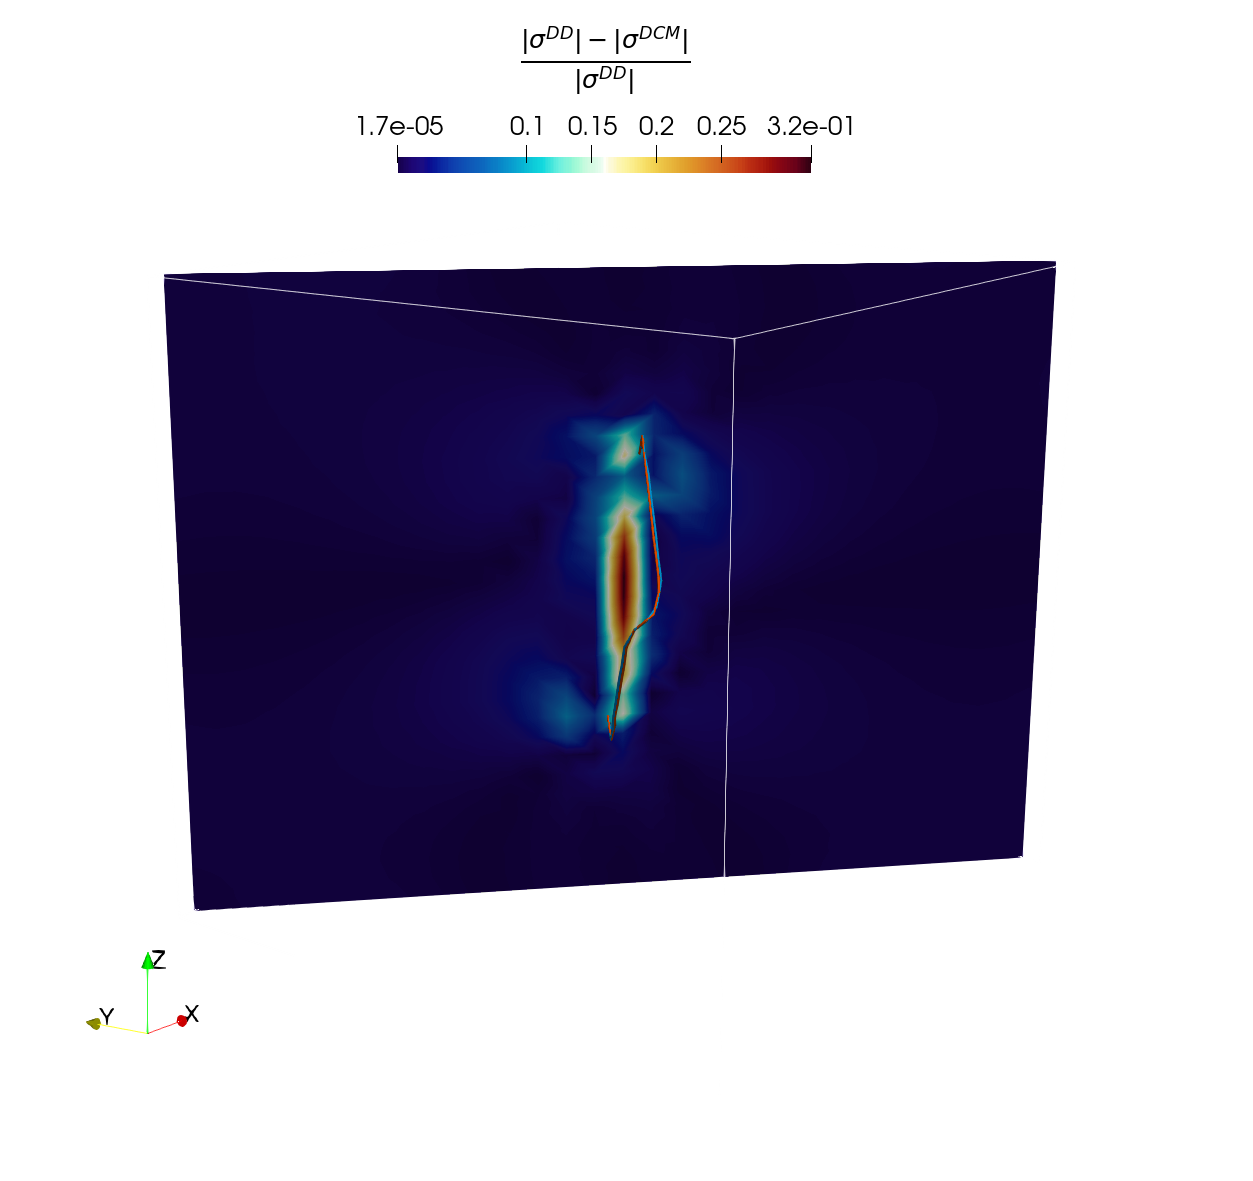
\includegraphics[height=0.6\textwidth]{pngFigures/final_disloc_stress.png}}
  % \caption{(\subref{subfig:microstructure}) Exemple de microstructure générée avec le logiciel \textsc{Neper} -- (\subref{subfig:ondePlane}) propagation d'une onde plane dans la microstructure \subref{subfig:microstructure}.}
  \caption{{\'E}volution d'une boucle prismatique $\vect{b}=3(\vect{e}_y - \vect{e}_x)$ dans un domaine soumis à une contrainte de cisaillement homogène $\sigma_{yz} = \sigma_d$. Comparaison entre la solution DD pure (ligne orange) et la solution DCM (ligne bleue).}
  \label{fig:comparisonDCM}
\end{figure}
Le couplage DD-FFT vise essentiellement à résoudre des problèmes sur des grilles très fines en profitant de la grande rapidité de calcul offerte par l'algorithme FFT.
Dans ces travaux, cette formulation de la DCM sera considérée en couplant les codes \textit{Amitex} \cite{Amitex_FFT} et \textit{Numodis} \cite{Numodis}, tous deux développés au CEA pour les parties FFT et DD respectivement.
Le premier objectif de mon postdoc a été de terminer le couplage des deux codes afin d'obtenir des premières comparaisons satisfaisantes avec la DD seule.

La figure \ref{fig:comparisonDCM} montre un exemple de résultats obtenus sur un problème simple à titre d'illustration.
On considère une boucle de dislocation prismatique dans un cristal cubique à faces centrées supposé infini et soumis à une contrainte de cisaillement homogène $\sigma_{yz}$.
Sous l'action de cette contrainte, la dislocation se déforme et on compare les solutions calculées par la DCM et la DD pour s'assurer de la cohérence du couplage DD--FFT mis en place.

Les différences qui apparaissent dans l'évolution de la boucle prismatique évaluée par la DCM ou la DD, bien que faibles, s'explique premièrement par le choix de la procédure de régularisation des déformations plastiques qui n'est pas unique \cite{jamond2016_DCM,VATTRE2014,Capolungo2021}.
Par ailleurs, la DCM implique plusieurs paramètres algorithmiques jouant sur l'étalement des déformations plastiques et sur la taille de la zone où la correction DD est calculée.
Tout l'intérêt de ces paramètres est de pouvoir assurer un équilibre entre précision et efficacité de l'approche DCM.
Toutefois, aucune analyse numérique n'a permis à ce jour de déterminer de valeurs optimales pour ces derniers.

Le premier objectif de mon travail est donc l'analyse numérique du schéma DCM afin d'extraire des valeurs optimales de ces coefficients, en analysant les équations dans un premier temps, et en recourant à des simulations dans un second temps.
% On considère ici une boucle de dislocation prismatique contenue dans le plan de normale $\vect{n} = \vect{e}_y - \vect{e}_x$ dans un cristal cubique à faces centrées dont les axes cristallographiques sont alignés avec le repère global.
% Le vecteur de Burgers de cette dislocation est $\vect{b}=3\vect{n}$, de sorte que la boucle ne peut se mouvoir que dans la direction $\vect{n}$.
% Le domaine est soumis à une contrainte de cisaillement $\sigma_{yz}$ et le déplacement de la dislocation sous l'effet de ce chargement est calculée par la DCM d'une part et la DD d'autre part pour comparaison.


% Bien que la DCM permet de calculer des solutions proches de celles de la DD, le choix de la procédure de régularisation des déformations plastiques utilisée n'est pas unique \cite{jamond2016_DCM,VATTRE2014,Capolungo2021}, ce qui peut conduire à une précision variable de la méthode.
% Par ailleurs, la définition de la zone dans laquelle la correction DD est calculée repose sur un certain nombre de paramètres algorithmiques inteviennent, ces derniers permettent de régler la taille du domaine dans lequel la correction DD est calculée.

% \cite{bertin2015_fft,Capolungo2021,VATTRE2014}

% \begin{itemize}
% \item Défauts d'irradiation à l'échelle atomique
% \item Influence de ces défauts sur la plasticité (à travers leur interaction avec les dislocations) et modification du comportement plastique à l'échelle mésoscopique
% \item Le lien entre ces interactions et les comportements macroscopiques (écrouissage, localisation, fragilisation) n'est toutefois pas encore complètement clair. De sorte que ce sujet fait l'objet de beaucoup de recherches mutli-échelle
% \item Une méthode numérique permettant de simuler ce genre de problème est la méthode des dislocations discrète ... (description)
% \item Cette dernière est néanmoins limitées pour des raisons de coûts de calcul, à des problèmes impliquant des petites dimensions du domaines d'étude.
% \item Récemment, une approche couplant la DDD avec des méthodes adaptées à l'échelle macroscopique (FEM, FFT, \textit{etc.}) a été proposée. Parler des aires balayées par les dislocations dont on déduit les déformations plastiques, qui sont étalées dans le maillage afin de régulariser la discontinuité du déplacement résultant du mouvement des dislocation. La résolution éléments finis apparaît alors comme une étape de relaxation visant à relaxer les déformations plastiques en tenant compte des conditions aux limites.
  % {\`A} cause de la régularisation, le champ de contrainte calculé par la méthode macroscopique peine à capturer la solution analytique dans le voisinage des dislocations (pour des distances de l'ordre de la taille du maillage).
  % On utilise alors la contrainte calculée par la DDD pour corriger la solution proche des dislocations.
% \end{itemize}


\paragraph{Objectifs:}
% $\newline$
% \begin{itemize}
% \item Terminer et valider le couplage
% \item Optimisation des paramètres de la méthode $\rightarrow$ analyse numérique (illustrer ça par des figures)
% \item Exploitation du modèle sur des simulations à grande échelle pour l'étude de l'effet des défauts d'irradiation sur l'écoulement plastique (modèle de comportement homogénéisé)
% \end{itemize}


\begin{itemize}
\item expliquer le contexte / la problématique
\item la méthode DCM et ses grands principes
\item mon travail là-dedans et les objectifs fixés/remplis à ce jour.
\end{itemize}
%%% Local Variables:
%%% mode: latex
%%% TeX-master: "main"
%%% End:
